\section{Materiais e Métodos}
\label{sec:materiais}

Esta seção apresenta os procedimentos metodológicos adotados para a condução da pesquisa, bem como os instrumentos utilizados para coleta e análise dos dados. A pesquisa caracteriza-se como um estudo empírico, quantitativo e comparativo, cujo objetivo é investigar se a inclusão do código-fonte influencia a avaliação da qualidade de descrições de ferramentas MCP. 


O fluxo metodológico adotado encontra-se resumido na Figura \ref{fig:metodologia}. O processo inicia-se com a coleta de repositórios MCP públicos, seguida pela extração das ferramentas e das informações sobre sua implementação. Em seguida, as ferramentas são avaliadas em dois cenários distintos: no primeiro, considerando as descrições em linguagem natural; no segundo, utilizando descrições enriquecidas com informações extraídas do código-fonte. Por fim, os resultados obtidos são organizados e submetidos a uma análise comparativa e estatística.

\begin{figure}[H]
    \centering
    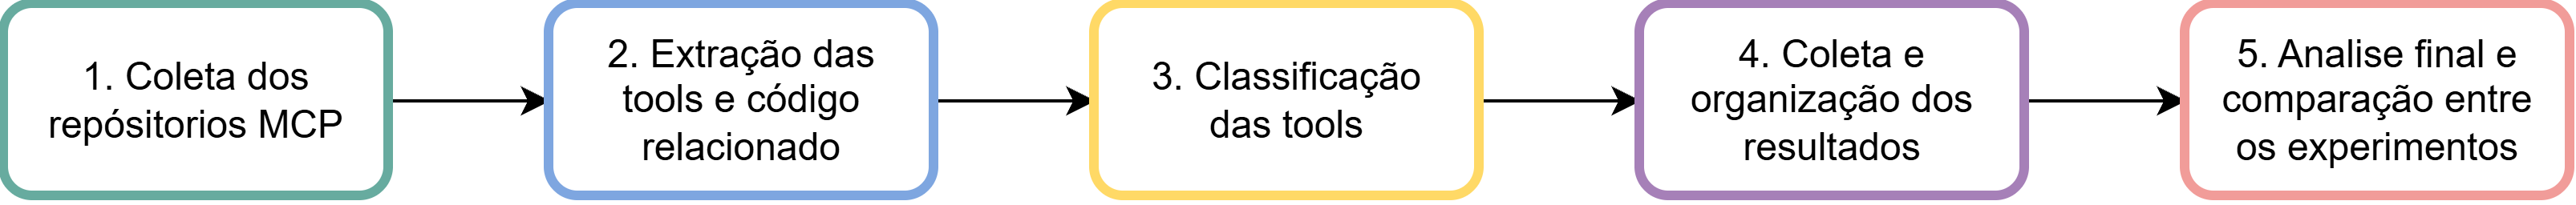
\includegraphics[width=1\linewidth]{./images/metodologia_v5.png}
    \caption{\textcolor{red}{Fluxo metodológico adotado na pesquisa}}
    \label{fig:metodologia}
\end{figure}

\subsection{Coleta dos Repositórios MCP}

A primeira etapa consiste na construção do conjunto de dados que servirá de base para os experimentos. Para isso, serão minerados repositórios públicos relacionados ao ecossistema MCP hospedados no GitHub. O objetivo dessa etapa é identificar implementações reais de servidores MCP que representem o cenário atual.

A coleta de dados será realizada por meio da API \textit{GraphQL} do GitHub, uma linguagem de consulta que permite recuperar estruturas de dados complexas de forma específica, minimizando as restrições impostas pelos limites de requisições da plataforma \cite{Brito2020}. As consultas retornarão apenas repositórios desenvolvidos em Python, JavaScript, TypeScript, Java ou C\# que não sejam classificados como \textit{forks}. 

Para garantir a relevância e a maturidade dos \textit{softwares} analisados, a coleta será restrita a repositórios que possuam \textcolor{red}{no mínimo} 100 estrelas (\textit{stars}). A adoção desse limiar fundamenta-se em estudos de mineração de repositórios que identificam o número de estrelas como uma medida direta de popularidade, sendo 100 estrelas um marco estatístico comum para filtrar projetos experimentais ou de baixo valor agregado, conhecidos como \textit{toy repositories} \cite{Borges2016}. Ao final, serão selecionados os 206 servidores mais populares, dobrando a amostra utilizada no estudo de Hasan et al. (2026)\nocite{2026arXiv260214878M} para ampliar a cobertura do ecossistema investigado.


\subsection{Extração das Ferramentas e do Código Relacionado}

Após a obtenção dos repositórios, será realizada a identificação automática das ferramentas disponibilizadas por cada servidor MCP. Para isso, será desenvolvido um algoritmo de mineração capaz de percorrer a estrutura dos projetos e localizar as implementações associadas às ferramentas expostas pelo servidor. Para cada ferramenta identificada, serão extraídos sua descrição em linguagem natural e sua localização no código-fonte.

Em seguida, será realizada a extração do código relacionado a cada ferramenta. Como os servidores MCP podem possuir arquiteturas distintas e envolver múltiplas camadas de abstração, a simples recuperação do método que registra uma ferramenta não é suficiente para representar adequadamente seu comportamento. Dessa forma, busca-se identificar não apenas o método diretamente associado à ferramenta, mas também os demais elementos do código-fonte que participam de sua execução. Para isso, será construída uma árvore de chamadas (\textit{call graph}) a partir do método responsável pela implementação da ferramenta. O método inicial será considerado o primeiro nível da árvore. Em seguida, serão identificados os métodos invocados diretamente por ele, compondo o segundo nível. Por fim, serão incluídos os métodos chamados pelos elementos do segundo nível, formando o terceiro nível da estrutura. Um exemplo desse processo é apresentado na Figura \ref{fig:codigoarvore}.

\begin{figure}[H]
    \centering
    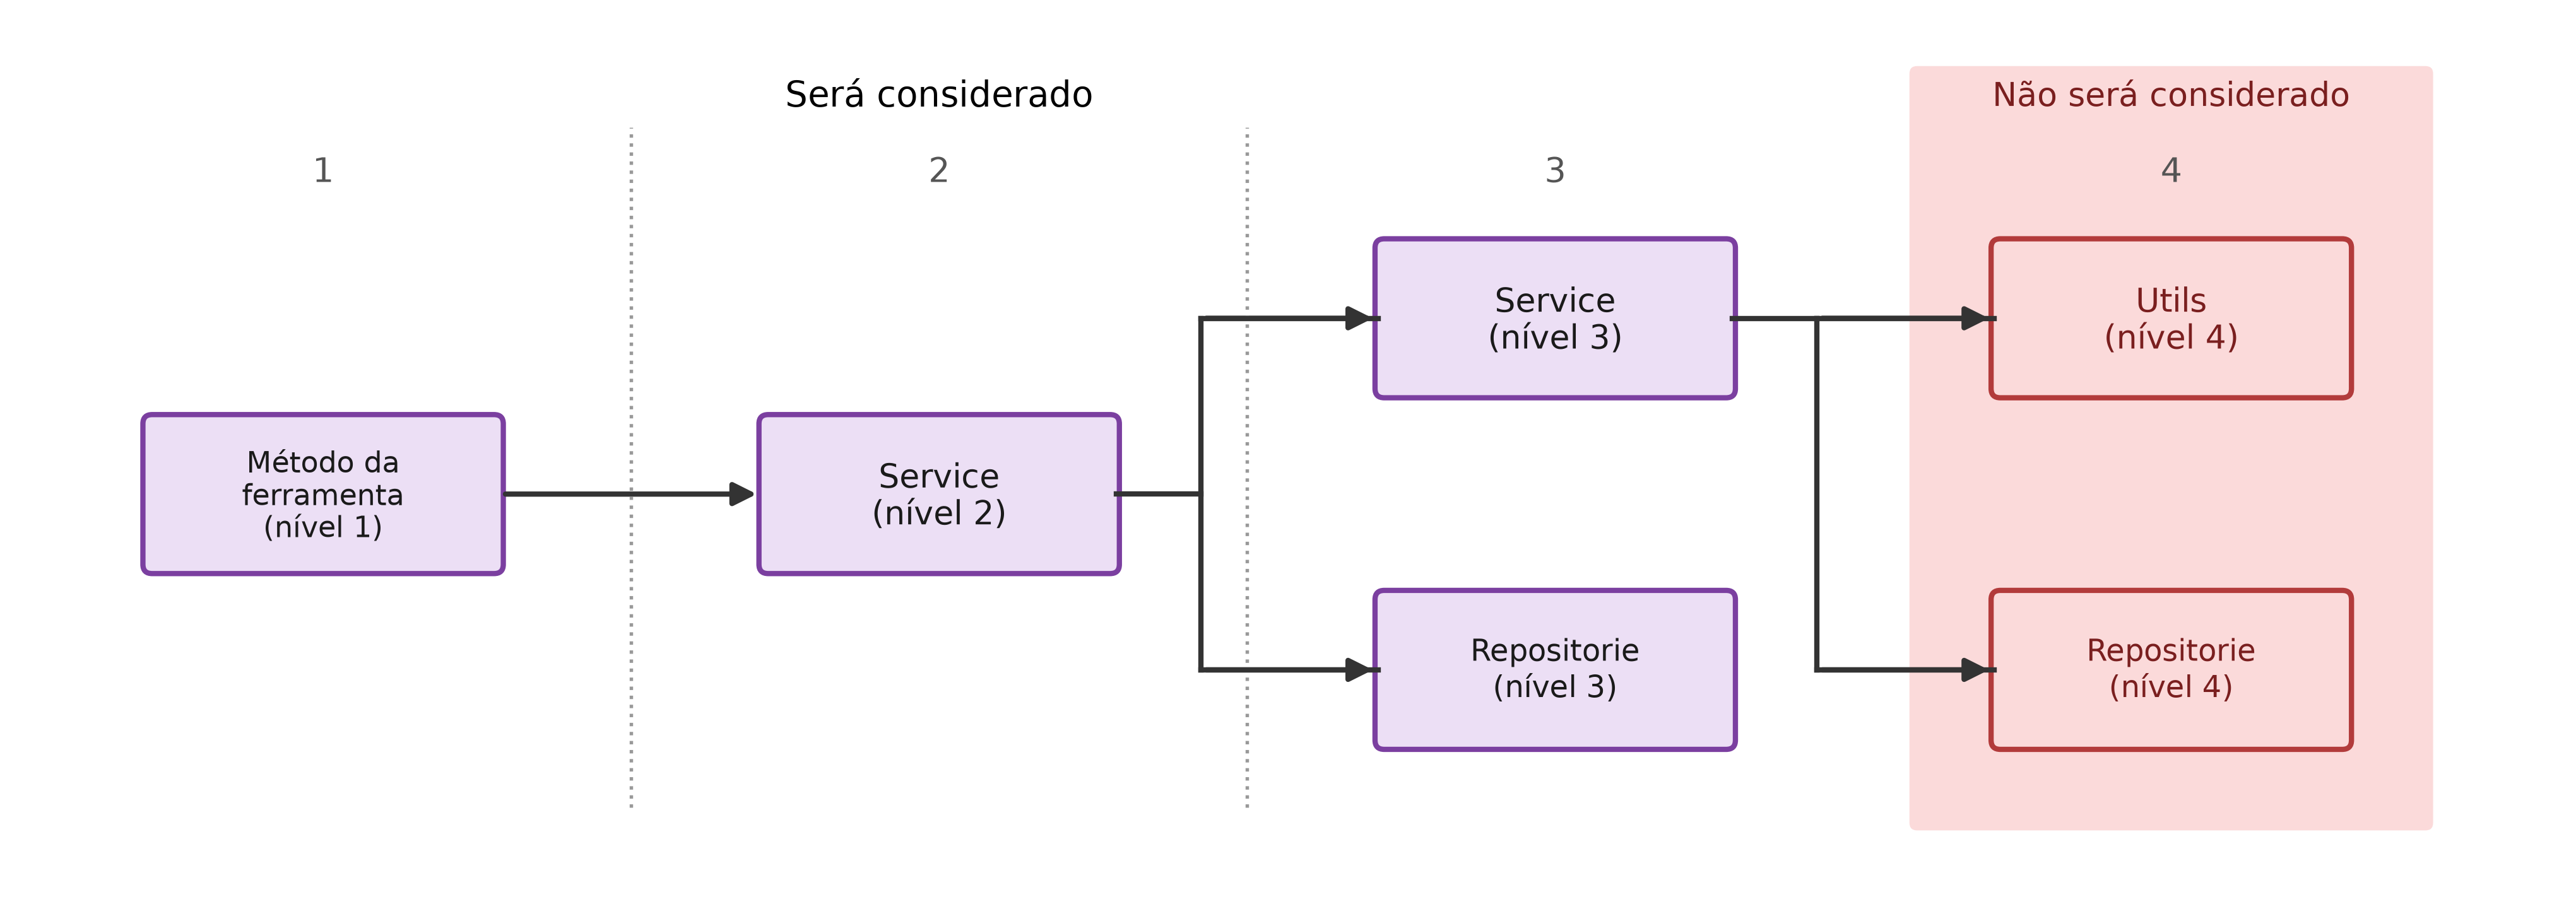
\includegraphics[width=1\linewidth]{./images/arvoreFinal.png}
    \caption{Exemplo de extração da árvore de chamadas de uma ferramenta}
    \label{fig:codigoarvore}
\end{figure}

Ao final desta etapa, será produzido um conjunto de dados estruturado contendo os servidores MCP analisados e as ferramentas identificadas em cada um deles. Para cada ferramenta, serão armazenadas sua descrição em linguagem natural e o conjunto de métodos obtido a partir da árvore de chamadas. Esse conjunto de dados servirá como entrada para as etapas subsequentes da pesquisa, nas quais as ferramentas dos repositórios coletados serão avaliadas  \textcolor{red}{quanto à qualidade de suas descrições, com e sem o uso do contexto do código-fonte correspondente.}

\subsection{Classificação das Ferramentas}

Na terceira etapa, \textcolor{red}{utilizando as \textit{tools} coletadas nas etapas anteriores, será conduzido um experimento comparativo estruturado em dois cenários de avaliação que serão executados em diferentes modelos de IA . No primeiro cenário, as descrições das ferramentas serão avaliadas com base em seu conteúdo em linguagem natural. No segundo, essas mesmas descrições serão avaliadas em conjunto com informações extraídas do código-fonte correspondente. Essa estratégia permite identificar o impacto da inclusão do contexto de implementação na avaliação da qualidade das descrições. A execução do cenário que combina descrição e código-fonte concretiza o objetivo específico (i)}.

Em ambos os cenários, a avaliação será conduzida com base na rubrica proposta por Hasan et al. (2026)\nocite{2026arXiv260214878M}, composta por seis componentes: \textit{Purpose}, que avalia a clareza com que a descrição comunica a finalidade da ferramenta; \textit{Guidelines}, que verifica se existem orientações sobre quando e como utilizá-la; \textit{Limitations}, que analisa a explicitação de restrições, premissas ou casos de falha; \textit{Parameter Explanation}, que mede a qualidade da documentação dos parâmetros de entrada; \textit{Length and Completeness}, que avalia o nível de detalhamento e cobertura da descrição; e \textit{Examples}, que verifica a presença de exemplos de utilização. Cada componente recebe uma pontuação em uma escala Likert de cinco pontos, sendo posteriormente utilizada para identificar deficiências associadas aos respectivos \textit{smells} descritos pelos autores.

No primeiro cenário, os modelos de linguagem atuarão como avaliadores (\textit{LLM-as-a-Judge}) recebendo as descrições das ferramentas. Nesse contexto, a classificação será realizada sem qualquer acesso à implementação da funcionalidade analisada. No segundo cenário, além da descrição da ferramenta, o modelo receberá, também, a representação estrutural obtida a partir da árvore de chamadas correspondente. Dessa forma, o avaliador poderá confrontar a documentação fornecida com aspectos observáveis da implementação, verificando a existência de omissões, inconsistências ou informações potencialmente enganosas que não seriam perceptíveis apenas pela análise da descrição.


\subsection{Organização dos Resultados}

Concluída a etapa de classificação, os resultados produzidos nos dois cenários experimentais serão coletados e estruturados em uma base de dados unificada. Para cada ferramenta analisada, serão armazenados identificadores que permitam sua associação ao servidor MCP de origem, bem como os resultados obtidos nos cenários com e sem a inclusão de informações provenientes do código-fonte\textcolor{red}{, além de qual modelo de IA foi utilizado para a analise.}

A base de dados resultante conterá os escores atribuídos pelo modelo para cada dimensão de qualidade avaliada, além das classificações finais produzidas em cada execução do experimento. Dessa forma, cada ferramenta possuirá dois conjuntos de resultados \textcolor{red}{por modelo que estarão diretamente vinculados} à mesma descrição, diferindo apenas pela presença ou ausência das informações extraídas do código-fonte. Essa organização permitirá estabelecer um relacionamento direto entre as avaliações realizadas sobre uma mesma ferramenta, preservando o pareamento necessário para as análises estatísticas subsequentes e possibilitando a comparação consistente dos resultados obtidos nos dois cenários experimentais.

\subsection{Análise Comparativa dos Experimentos}

Na etapa final, os resultados obtidos serão analisados com o objetivo de identificar diferenças entre os dois cenários de avaliação. \textcolor{red}{Essa análise busca validar se a utilização do código-fonte de fato altera os resultados da avaliação das descrições, além de identificar quais atributos da rubrica utilizada para avaliar a qualidade são mais e menos impactados pela adição do código-fonte.}

Inicialmente, será realizada uma análise \textcolor{red}{por meio do cálculo de medidas como média, mediana e desvio-padrão dos escores atribuídos a cada dimensão de qualidade avaliada, para identificar se houve diferença numérica nos resultados gerados com e sem o contexto do código-fonte das ferramentas MCP, atendendo ao objetivo específico (ii) desta pesquisa. A partir dessa comparação, será possível avaliar quais atributos foram mais afetados pela inserção do contexto técnico. Será realizado também} o Teste de Postos Sinalizados de Wilcoxon \cite{wilcoxon1945individual}, aplicado individualmente para cada dimensão de qualidade, a fim de verificar se as diferenças observadas entre as avaliações são estatisticamente significativas, \textcolor{red}{concluindo o objetivo específico (iii). O teste será aplicado separadamente para cada modelo de linguagem utilizado, permitindo verificar se o efeito da inclusão do código-fonte se mantém consistente entre diferentes avaliadores.} Como as duas avaliações são realizadas sobre a mesma ferramenta, o teste é adequado por considerar amostras pareadas e não exigir a suposição de normalidade dos dados. \textcolor{red}{Os resultados dessa análise fornecerão as evidências empíricas necessárias para apoiar ou refutar a hipótese de que a incorporação do contexto técnico amplia a capacidade de detecção de \textit{smells} em descrições de ferramentas MCP.}

\subsection{Distribuição de Tarefas e Cronograma (TCC II)}
Por tratar-se de um trabalho desenvolvido em dupla, a execução das atividades durante o TCC II foi planejada para operar de forma paralela e complementar, assegurando que ambos os integrantes assumam protagonismo em frentes distintas de desenvolvimento e análise. O aluno Pedro Henrique Pires Rodrigues assumirá a frente de infraestrutura e integração, sendo o responsável por configurar a infraestrutura de extração, implementar a configuração do \textit{LLM-as-a-Judge} e conduzir os testes pilotos com ajustes de parâmetros.

Simultaneamente, o aluno Vinicius Rezende Arantes de Araujo Moreira focará na mineração de dados e na lógica estrutural, responsabilizando-se pelo desenvolvimento do algoritmo via GraphQL e pela implementação da extração profunda da árvore de código (\textit{call graph}). \textcolor{red}{Adicionalmente, Vinicius realizará a consolidação tabular das métricas junto às análises estatísticas iniciais. A etapa de classificação das ferramentas, contemplando os dois cenários de avaliação, será conduzida conjuntamente pelos dois integrantes.}

A condução do cronograma seguirá um modelo de progresso contínuo, com a maior parte das tarefas técnicas executadas de forma individual entre agosto e outubro. A partir do mês de novembro, a dupla atuará de forma conjunta na discussão detalhada dos resultados, na redação da conclusão e na revisão final de coerência e formatação do artigo. A Tabela \ref{tab:datas} explicita a alocação de esforço por indivíduo e por quinzena para o semestre de 2026.


\begin{table}[H]
\centering
\caption{Distribuição de tarefas paralelas e conjuntas por quinzenas (TCC II - 2026)}
\label{tab:datas}
\resizebox{\textwidth}{!}{%
\begin{tabular}{|l|c|c|c|c|c|c|c|c|c|}
\hline
\multirow{2}{*}{\textbf{Tarefas}} & \multirow{2}{*}{\textbf{Responsável}} & \multicolumn{2}{c|}{\textbf{Agosto}} & \multicolumn{2}{c|}{\textbf{Setembro}} & \multicolumn{2}{c|}{\textbf{Outubro}} & \multicolumn{2}{c|}{\textbf{Novembro}} \\ \cline{3-10} 
 &  & \textbf{1ªQ} & \textbf{2ªQ} & \textbf{1ªQ} & \textbf{2ªQ} & \textbf{1ªQ} & \textbf{2ªQ} & \textbf{1ªQ} & \textbf{2ªQ} \\ \hline
Configuração da Infraestrutura de Extração de Dados & Pedro & X &  &  &  &  &  &  &  \\ \hline
Desenvolvimento do algoritmo de mineração via GraphQL & Vinicius & X & X &  &  &  &  &  &  \\ \hline
Integração e configuração do \textit{LLM-as-a-Judge} & Pedro & X & X & X &  &  &  &  &  \\ \hline
Implementação do algoritmo de \textit{Call Graph} & Vinicius &  &  & X & X &  &  &  &  \\ \hline
Execução de teste piloto e ajuste de parâmetros & Pedro &  &  &  & X &  &  &  &  \\ \hline
Aplicação da Avaliação & Ambos &  &  &  &  & X & X &  &  \\ \hline
Consolidação tabular e análises estatísticas & Vinicius &  &  &  &  &  &  & X &  \\ \hline
Discussão de Resultados e Conclusão & Ambos &  &  &  &  &  &  & X & X \\ \hline
Revisão textual, coerência e formatação final & Ambos &  &  &  &  &  &  &  & X \\ \hline
\end{tabular}%
}
\end{table}